\chapter{TỔNG QUAN VỀ DỰ ÁN VÀ CƠ SỞ LÝ THUYẾT}

\section{Giới thiệu dự án Website Cửa hàng Tiện lợi 7coMART}

\subsection{Bối cảnh dự án}
Trong kỷ nguyên số hóa và sự bùng nổ của mô hình thương mại điện tử giao hàng tức thì (Quick Commerce), việc vận hành một hệ thống cửa hàng tiện lợi trực tuyến đòi hỏi tính ổn định và tốc độ xử lý giao dịch thời gian thực cao. Dự án website cửa hàng tiện lợi \textbf{7coMART} được thiết kế nhằm đáp ứng nhu cầu mua sắm nhu yếu phẩm nhanh chóng của khách hàng trực tuyến, tích hợp các tính năng đặt hàng, quản lý danh mục và phân bổ kho hàng tự động.

\subsection{Kiến trúc kỹ thuật của hệ thống}
Hệ thống 7coMART được xây dựng dựa trên những công nghệ hiện đại, đảm bảo hiệu năng và khả năng mở rộng:
\begin{itemize}
    \item \textbf{Frontend (Giao diện người dùng):} ReactJS kết hợp với TypeScript giúp xây dựng giao diện Single Page Application (SPA) mượt mà, phản hồi nhanh và tối ưu hóa trải nghiệm người dùng trên cả thiết bị di động lẫn máy tính để bàn.
    \item \textbf{Backend (Xử lý nghiệp vụ):} Python FastAPI cung cấp hệ thống API RESTful hiệu năng cực cao nhờ cơ chế bất đồng bộ (async-first), tự động sinh tài liệu kiểm thử tương tác Swagger UI thuận tiện cho việc phát hiện lỗi.
    \item \textbf{Database (Lưu trữ dữ liệu):} PostgreSQL 16 đóng vai trò cơ sở dữ liệu quan hệ chính, đảm bảo tính toàn vẹn dữ liệu giao dịch nhờ cơ chế ACID nghiêm ngặt.
    \item \textbf{Caching \& Locking:} Redis 7 được tích hợp để lưu trữ cache giỏ hàng tạm thời và thực hiện cơ chế khóa bi quan (Pessimistic Locking) ngăn chặn hiện tượng bán quá mức (overselling) khi có nhiều khách hàng mua cùng một mặt hàng tại một thời điểm.
    \item \textbf{Triển khai:} Đóng gói toàn bộ hệ thống bằng Docker Compose giúp đồng bộ môi trường phát triển và kiểm thử.
\end{itemize}

\subsection{Các mô-đun chức năng cốt lõi}
Hệ thống tập trung vào 4 luồng nghiệp vụ lớn của khách hàng:
\begin{enumerate}
    \item \textbf{Mô-đun Xác thực (Authentication):} Cho phép người dùng đăng ký tài khoản, đăng nhập hệ thống, quản lý thông tin cá nhân. Phân quyền truy cập rõ ràng dựa trên JWT Token giữa các vai trò: Khách hàng (Customer), Nhân viên quản lý đơn hàng (Staff) và Quản trị viên (Admin).
    \item \textbf{Mô-đun Danh mục và Sản phẩm (Catalog Search):} Hiển thị danh sách sản phẩm trực quan, hỗ trợ tìm kiếm sản phẩm theo tên và lọc theo các danh mục như thực phẩm, đồ uống, hóa mỹ phẩm.
    \item \textbf{Mô-đun Giỏ hàng (Cart):} Hỗ trợ thêm sản phẩm, cập nhật số lượng trực tiếp trong giỏ hàng, đồng bộ hóa thời gian thực và tính toán giá trị tạm tính của đơn hàng.
    \item \textbf{Mô-đun Đặt hàng và Xử lý kho (Order Processing):} Thực hiện lưu vết đơn hàng, phân bổ kho hàng tự động áp dụng thuật toán FEFO (First Expired First Out - Lô hàng hết hạn trước xuất trước) nhằm tối ưu hóa việc quản lý hạn sử dụng của sản phẩm tiện lợi.
\end{enumerate}

% =========================================================================
% HƯỚNG DẪN CHÈN ẢNH CHO SINH VIÊN:
% Bạn hãy chạy project 7coMART, chụp ảnh màn hình trang chủ bán hàng (http://localhost),
% lưu ảnh đó thành file '7comart_homepage.png' (hoặc .jpg) và bỏ vào thư mục:
% Test_Report/figs/
% Sau đó thay thế tên file bên dưới nếu định dạng ảnh khác png.
% =========================================================================
\begin{figure}[H]
    \centering
    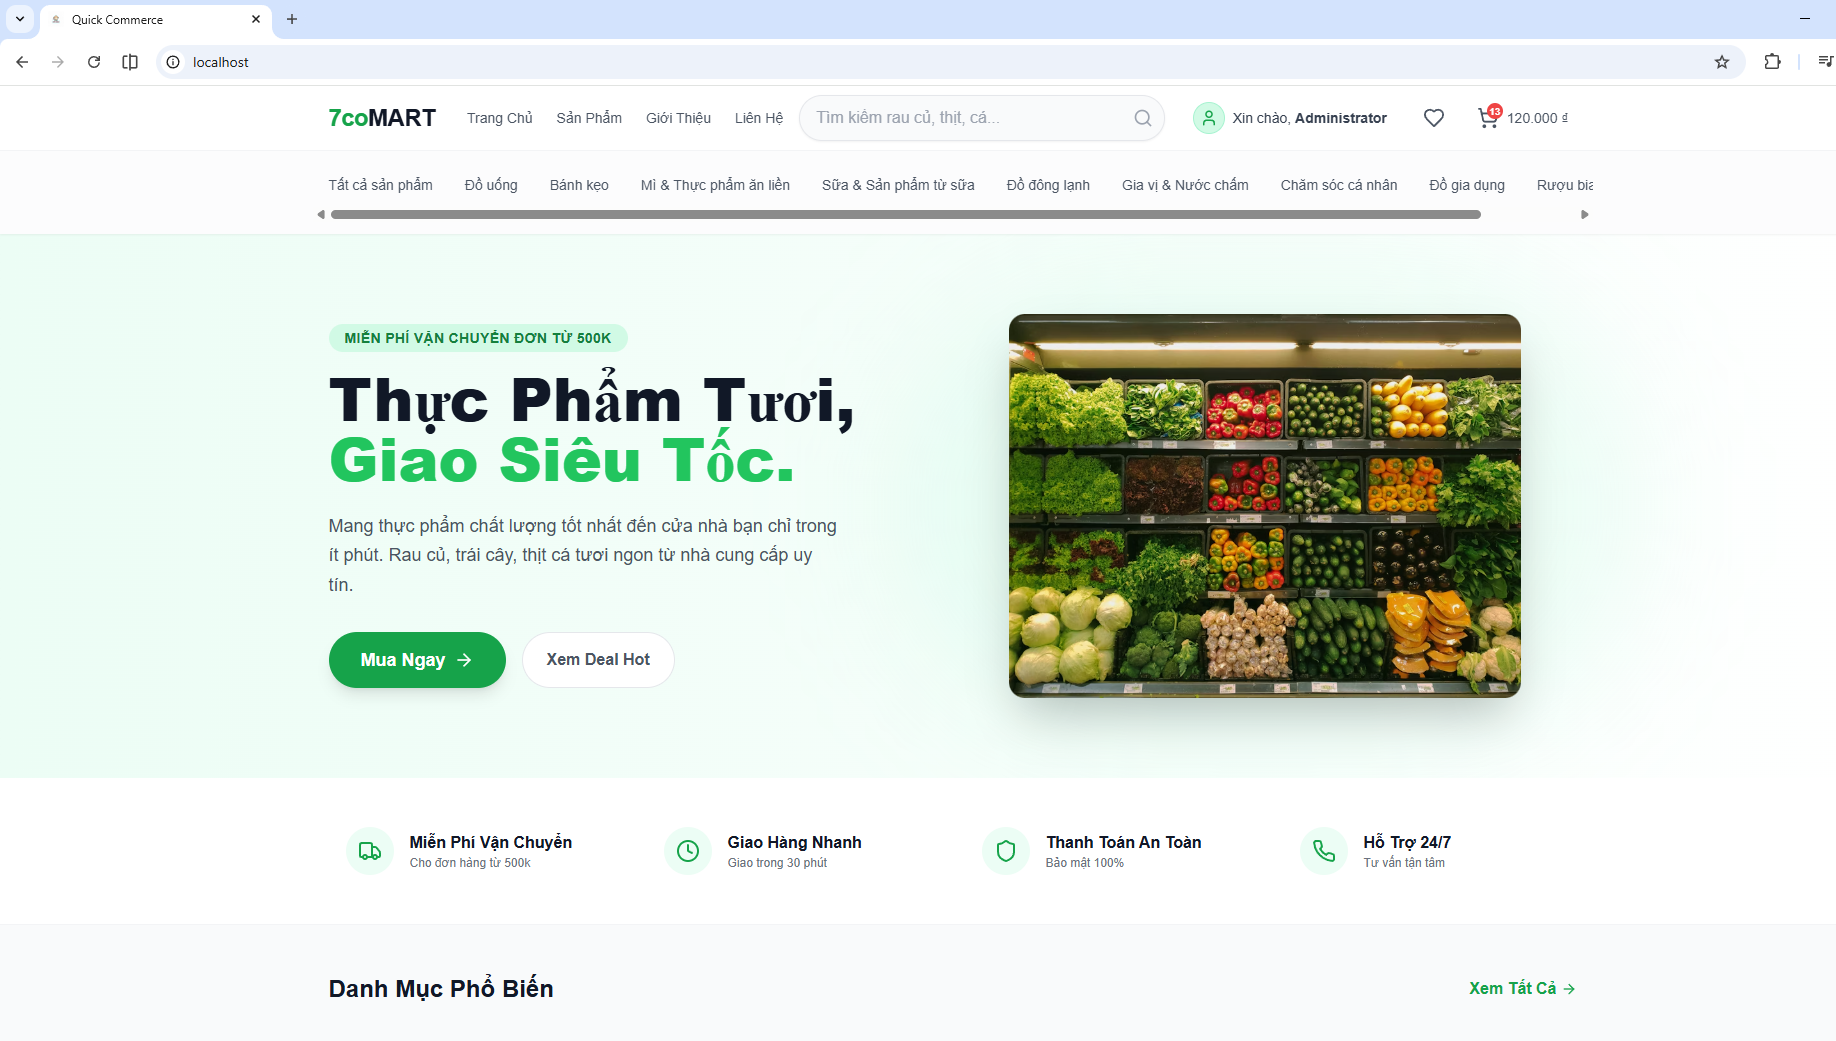
\includegraphics[width=0.85\textwidth]{figs/homepage.png}
    \caption{Giao diện trang chủ mua sắm trực tuyến của hệ thống cửa hàng tiện lợi 7coMART}
    \label{fig:7comart_homepage}
\end{figure}

\textbf{Nhận xét giao diện:} Như được minh họa tại Hình \ref{fig:7comart_homepage}, giao diện trang chủ của 7coMART được thiết kế hiện đại, responsive hoàn toàn. Các khối danh mục sản phẩm tiện lợi được bố trí trực quan giúp người dùng dễ dàng tìm kiếm và lựa chọn sản phẩm nhanh chóng. Ô tìm kiếm nổi bật ở thanh Header là tiêu điểm cho các kịch bản kiểm thử tìm kiếm tiếp theo.

\section{Tổng quan về Kiểm thử phần mềm}

\subsection{Mục tiêu và Tầm quan trọng}
Kiểm thử phần mềm là quá trình khảo sát thực nghiệm một sản phẩm phần mềm nhằm cung cấp cho các bên liên quan thông tin về chất lượng của sản phẩm đó. Đối với 7coMART, kiểm thử phần mềm giúp:
\begin{itemize}
    \item Phát hiện sớm các lỗi logic nghiệp vụ trong việc tính tiền giỏ hàng, trừ kho hàng FEFO trước khi hệ thống chính thức vận hành thương mại.
    \item Đảm bảo an toàn bảo mật, chống các cuộc tấn công đánh cắp tài khoản hoặc can thiệp tham số giá tiền.
    \item Khẳng định hệ thống chạy đúng yêu cầu đặc tả chức năng và đem lại trải nghiệm mua sắm ổn định nhất cho người dùng.
\end{itemize}

\subsection{Áp dụng 7 nguyên tắc kiểm thử phần mềm vào dự án 7coMART}
\begin{enumerate}
    \item \textbf{Kiểm thử chỉ ra sự hiện diện của lỗi (Testing shows presence of defects):} Các kịch bản kiểm thử được thiết kế nhằm tìm kiếm và chứng minh website 7coMART vẫn tồn tại lỗi (như lỗi SQLi, lỗi số lượng âm). Kiểm thử không thể chứng minh hệ thống hoàn hảo 100\% không có lỗi.
    \item \textbf{Kiểm thử toàn diện là bất khả thi (Exhaustive testing is impossible):} Số lượng sản phẩm kết hợp trong giỏ hàng và dữ liệu nhập vào form là vô hạn. Nhóm tập trung thiết kế các kịch bản kiểm thử trọng tâm cho luồng mua sắm chính bằng cách phân lớp dữ liệu.
    \item \textbf{Kiểm thử càng sớm càng tốt (Early testing):} Việc lập kế hoạch và thiết kế kịch bản test được nhóm triển khai ngay sau khi chốt tài liệu đặc tả yêu cầu chức năng, giúp phát hiện lỗi logic ngay trên bản thiết kế trước khi lập trình viên bắt tay viết code.
    \item \textbf{Sự tập trung của lỗi (Defects clustering):} Lỗi thường tập trung nhiều ở những mô-đun phức tạp. Trong 7coMART, lỗi chủ yếu nằm ở mô-đun đặt hàng kết hợp với khóa đồng thời trừ kho PostgreSQL và kiểm soát hạn sử dụng.
    \item \textbf{Nghịch lý thuốc trừ sâu (Pesticide paradox):} Nếu liên tục lặp lại một bộ test cases cũ, nhóm sẽ không tìm thêm được lỗi mới. Vì vậy, bộ kịch bản test luôn được cập nhật, bổ sung các ca kiểm thử biên và giá trị ngẫu nhiên.
    \item \textbf{Kiểm thử phụ thuộc vào ngữ cảnh (Testing is context dependent):} 7coMART is một ứng dụng thương mại điện tử, do đó ngữ cảnh kiểm thử cực kỳ coi trọng tính toàn vẹn dữ liệu giỏ hàng, giao dịch đặt hàng và tính bảo mật của mã hóa mật khẩu.
    \item \textbf{Sự ngộ nhận về việc không có lỗi (Absence-of-errors fallacy):} Một hệ thống 7coMART được test sạch bóng lỗi kỹ thuật vẫn là thất bại nếu giao diện quá khó dùng, luồng đặt hàng rườm rà khiến khách hàng bỏ đi. Nhóm luôn kiểm định dựa trên trải nghiệm khách hàng thực tế.
\end{enumerate}

\subsection{Phân biệt Kiểm thử Chức năng và Kiểm thử Phi chức năng}
\begin{table}[H]
\centering
\caption{So sánh Kiểm thử Chức năng và Phi chức năng tại 7coMART}
\renewcommand{\arraystretch}{1.3}
\begin{tabular}{|p{2.2cm}|p{6cm}|p{6cm}|}
\hline
\textbf{Tiêu chí} & \textbf{Kiểm thử Chức năng} & \textbf{Kiểm thử Phi chức năng} \\ \hline
\textbf{Mục tiêu} & Kiểm tra hệ thống làm ĐÚNG chức năng yêu cầu hay không. & Kiểm tra hệ thống hoạt động TỐT như thế nào (hiệu năng, bảo mật). \\ \hline
\textbf{Đối tượng} & Đăng nhập thành công, tìm thấy sản phẩm, thêm đúng số lượng giỏ hàng, tạo đơn hàng trừ kho đúng lô FEFO. & Thời gian phản hồi API dưới 200ms, mã hóa mật khẩu bằng bcrypt, chống tấn công SQLi, XSS. \\ \hline
\textbf{Công cụ} & Manual test trên trình duyệt, Postman gọi API. & JMeter (tải), OWASP ZAP (bảo mật), Lighthouse. \\ \hline
\end{tabular}
\end{table}

\section{Tổng quan về công cụ quản lý lỗi Mantis Bug Tracker}
Mantis Bug Tracker (MantisBT) là một hệ thống theo dõi lỗi phần mềm mã nguồn mở dựa trên web. Công cụ cung cấp một quy trình chuyên nghiệp giúp Tester ghi nhận lỗi một cách chi tiết và phân công cho Lập trình viên xử lý, theo sát vòng đời lỗi từ lúc phát hiện cho tới khi được khắc phục hoàn toàn. Sự tích hợp Mantis giúp tăng cường tính minh bạch, rút ngắn khoảng cách giao tiếp giữa các thành viên dự án và tự động hóa các đo lường báo cáo chất lượng phần mềm.